\documentclass{article}\usepackage[]{graphicx}\usepackage[]{color}
%% maxwidth is the original width if it is less than linewidth
%% otherwise use linewidth (to make sure the graphics do not exceed the margin)
\makeatletter
\def\maxwidth{ %
  \ifdim\Gin@nat@width>\linewidth
    \linewidth
  \else
    \Gin@nat@width
  \fi
}
\makeatother

\definecolor{fgcolor}{rgb}{0.345, 0.345, 0.345}
\newcommand{\hlnum}[1]{\textcolor[rgb]{0.686,0.059,0.569}{#1}}%
\newcommand{\hlstr}[1]{\textcolor[rgb]{0.192,0.494,0.8}{#1}}%
\newcommand{\hlcom}[1]{\textcolor[rgb]{0.678,0.584,0.686}{\textit{#1}}}%
\newcommand{\hlopt}[1]{\textcolor[rgb]{0,0,0}{#1}}%
\newcommand{\hlstd}[1]{\textcolor[rgb]{0.345,0.345,0.345}{#1}}%
\newcommand{\hlkwa}[1]{\textcolor[rgb]{0.161,0.373,0.58}{\textbf{#1}}}%
\newcommand{\hlkwb}[1]{\textcolor[rgb]{0.69,0.353,0.396}{#1}}%
\newcommand{\hlkwc}[1]{\textcolor[rgb]{0.333,0.667,0.333}{#1}}%
\newcommand{\hlkwd}[1]{\textcolor[rgb]{0.737,0.353,0.396}{\textbf{#1}}}%
\let\hlipl\hlkwb

\usepackage{framed}
\makeatletter
\newenvironment{kframe}{%
 \def\at@end@of@kframe{}%
 \ifinner\ifhmode%
  \def\at@end@of@kframe{\end{minipage}}%
  \begin{minipage}{\columnwidth}%
 \fi\fi%
 \def\FrameCommand##1{\hskip\@totalleftmargin \hskip-\fboxsep
 \colorbox{shadecolor}{##1}\hskip-\fboxsep
     % There is no \\@totalrightmargin, so:
     \hskip-\linewidth \hskip-\@totalleftmargin \hskip\columnwidth}%
 \MakeFramed {\advance\hsize-\width
   \@totalleftmargin\z@ \linewidth\hsize
   \@setminipage}}%
 {\par\unskip\endMakeFramed%
 \at@end@of@kframe}
\makeatother

\definecolor{shadecolor}{rgb}{.97, .97, .97}
\definecolor{messagecolor}{rgb}{0, 0, 0}
\definecolor{warningcolor}{rgb}{1, 0, 1}
\definecolor{errorcolor}{rgb}{1, 0, 0}
\newenvironment{knitrout}{}{} % an empty environment to be redefined in TeX

\usepackage{alltt}

\usepackage{amsmath, amssymb}
\usepackage{graphicx}
\usepackage{hyperref}
\usepackage{listings}
\IfFileExists{upquote.sty}{\usepackage{upquote}}{}
\begin{document}

\title{Pol Sci 630:  Problem Set 12: 2SLS, RDD, ggplot2}

\author{Prepared by: Anh Le (\href{mailto:anh.le@duke.edu}{anh.le@duke.edu})}

\date{Due Date: Wed, Nov 23, 2016 (Beginning of Class)}

\maketitle

\section{2SLS}

\textbf{\color{red} Insert your comments on the assignment that you are grading above the solution in bold and red text. For example write: "GRADER COMMENT: everything is correct! - 8/8 Points" Also briefly point out which, if any, problems were not solved correctly and what the mistake was. See below for more examples.}

\subsection{Load dataset CigarettesSW from package AER}

\begin{knitrout}
\definecolor{shadecolor}{rgb}{0.969, 0.969, 0.969}\color{fgcolor}\begin{kframe}
\begin{alltt}
\hlkwd{library}\hlstd{(AER)}
\hlkwd{data}\hlstd{(}\hlstr{"CigarettesSW"}\hlstd{)}
\end{alltt}
\end{kframe}
\end{knitrout}

\subsection{Plot the following using ggplot2}

What can we say about the relationship between tax, price, and packs? Importantly, could sales tax be a valid instrument here? Explain your reasoning.

Note: This is a good way to show the relationship between 3 variables with a 2D plot.

\begin{knitrout}
\definecolor{shadecolor}{rgb}{0.969, 0.969, 0.969}\color{fgcolor}
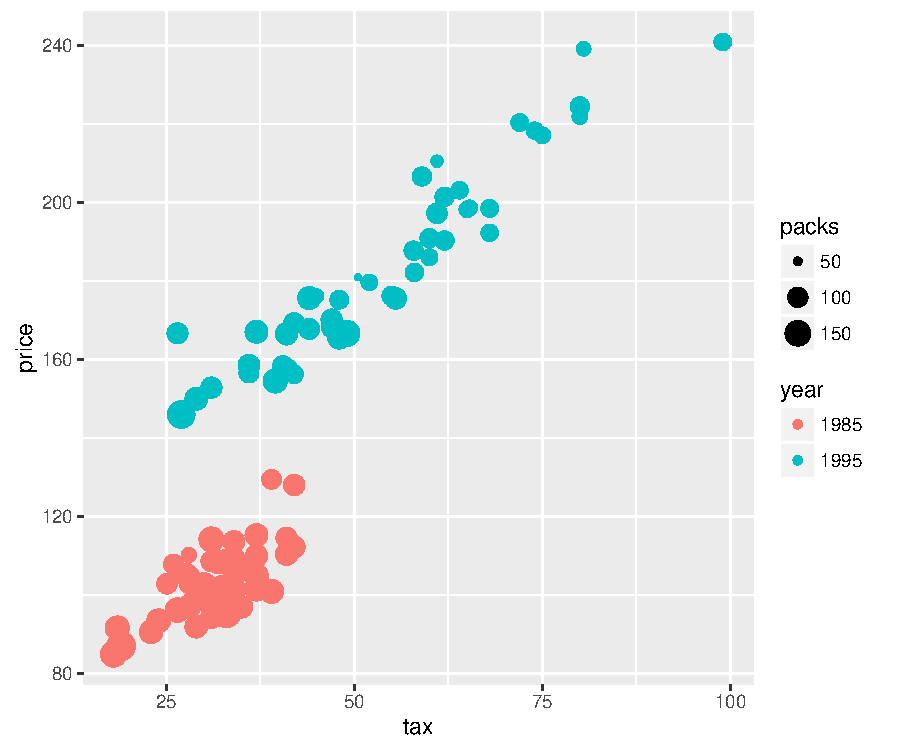
\includegraphics[width=\maxwidth]{figure/unnamed-chunk-2-1} 

\end{knitrout}

\subsection{Divide variable income by 1000 (for interpretability)}

\subsection{Run 2SLS}

Run 2SLS with \verb`ivreg`. Outcome: packs. Exogenous var: income. Endogenous var: price, whose instrument is tax. Interpret the coefficient of \verb`income` and \verb`price`.

Note: Different from the model during lab, this model has an exogenous independent variable that doesn't need to be instrumented for. See `help(ivreg)` $>$ Details, which explains how to deal with this.

\subsection{2SLS diagnostics: use F-test to check for weak instrument}

\subsection{2SLS by hand}

Run the 2SLS by hand, i.e. not using \verb`ivreg`, but run 2 stages of \verb`lm`. Do you get the same estimate from \verb`ivreg`?

\subsection{Weak instrument test by hand}

The weak instrument test aims to test whether the instrument is an important predictor of the endogenous variables, even after controlling for other variables.

We do it as follows:

\begin{itemize}
\item Run the standard 1st stage regression of endogenous var ~ instrument + exogenous vars
\item Run a ``modified'' 1st stage regression of endogenous var ~ exogenous vars
\item Use \verb`waldtest(model1, model2)` to compare the two models (to see if the model with the instrument fits better). The null hypothesis is that the instrument has a statistically significant impact
\end{itemize}
The rule of thumb is that the F-statistic should be $>$ 10

Implement the weak instrument test as described above and show that it gets the same F-statistic as given by \verb`ivreg`.

\section{Regression Discontinuity Design}

Find the replication data here \url{https://dataverse.harvard.edu/dataset.xhtml?persistentId=doi:10.7910/DVN/9OOLQ7}

\begin{knitrout}
\definecolor{shadecolor}{rgb}{0.969, 0.969, 0.969}\color{fgcolor}\begin{kframe}
\begin{alltt}
\hlcom{# Load the data like this}
\hlcom{# load("replication_data.RData")}
\end{alltt}
\end{kframe}
\end{knitrout}

Variables that you'll use: elecpopratio (\% of the population as the electorate), treat (whether got audited or not), electorate.perpop07 (\% registration in 07), electorate.perpop08 (\% registration in 08)

Read (by which I mean Ctrl + F) through the paper to figure out which bandwidth and the cutoff points the authors used. Read help(rdrobust) to see how to specify our own bandwidth and cutoff points.

In this exercise we'll replicate their main results in Table 2 (p. 447)

\subsection{Sharp RDD}

Use rdrobust to estimate the RDD effect of elecpopratio $>$ 0.8 for Change in registration (\%) ($\hat\tau_A$ in Table 2), using 1) the author's bandwidth, and 2) the bandwidth chosen by rdrobust itself.

\subsection{Fuzzy RDD}

The design of this paper is a Fuzzy RDD because when elecpopratio $>$ 0.8, a district may be audited but not necessarily.

rdrobust has an argument \verb`fuzzy` to specify which observation is actually treated. Use it to get a Fuzzy RDD estimate for Change in registration (\%) ($\hat\tau_R$ in Table 2)

\subsection{Density test (graphical)}

Plot the histogram of the number of observations on both sides of the cut-off to see if there's any difference

\end{document}
